\documentclass[asd-beamer.tex]{subfiles}

\begin{document}

\section{Variabili casuali e assiomi probabilit\'a}

\subsection{Assiomi di probabilit\'a}\linkdest{axioms}

\begin{frame}{Assiomi probabilit\'a Kolmogorov: spazio di probabilit\'a $(\Omega,F,P)$}
$\Omega$ spazio campionario (sample space: $\{1,2,3,4,5,6\}$) , $F$ (: (1), (dado pari), etc) 
\begin{itemize}
\item Spazio campionario: set enumerating each and every possible outcomes (simple events) of experiment. La probabilit\'a di un evento \'e $\prob{(E)}\geq0$ per ogni $E\in S$ spazio campionario.
\item La probabilit\'a degli eventi del sample space \'e 1.
\item $\sigma$-additivit\'a: per ogni sequenza numerabile di insiemi disgiunti (eventi mutualmente esclusivi)
\begin{equation*}
\prob{(\cup_{i=1}^{\infty}E_i)}=\sum_{i=1}^{\infty}\prob{(E_i)}
\end{equation*}
\end{itemize}
\begin{columns}[T]
	\begin{column}{0.5\textwidth}
\begin{block}{Addition rule: probability that A or B will}
\begin{equation*}
\prob{(A\cup B)}=\prob{(A)}+\prob{(B)}-\prob{(A\cap B)}
\end{equation*}
\end{block}
\end{column}
\begin{column}{0.5\textwidth}
\begin{block}{Teorema probabilit\'a totale}
$B_n$ partition of sample space
\begin{align*}
&\prob{(A)}=\sum_i\prob{(A\cup B_i)}\\
&=\sum_i\prob{(A|B_i)}\prob{(B_i)}
\end{align*}
\end{block}
\end{column}
\end{columns}
\end{frame}

\begin{frame}{Eventi congiunti}
\begin{columns}[T]
	\begin{column}{0.3\textwidth}
		\begin{block}{Probabilit\'a condizionata}
			\[\prob{(B|A)}=\frac{\prob{(B\cap A)}}{\prob{(A)}}
			\]
		\end{block}
	\end{column}
	\begin{column}{0.4\textwidth}
		\begin{block}{Teorema di Bayes}
			\[\prob{(A|B)}=\frac{\prob{(B|A)}\prob{(A)}}{\prob{(B)}}\]
		\end{block}
	\end{column}
	\begin{column}{0.25\textwidth}
		\begin{block}{eventi indipendenti}
			\[P(A|B)=P(A)\]
		\end{block}
	\end{column}
\end{columns}
\begin{columns}[T]\begin{column}{0.5\textwidth}
\begin{block}{\keyword{Eventi congiunti}}
$([x,x+dx],y)=(A)$: \keyword{marginal pdf} for x $\prob{(A)}=\int f(x,y)\,dxdy=f_x(x)\,dx$, $(x,[y,y+dy])=(B)$. $\prob{(A\cap B)}=f(x,y)\,dx\,dy$
\end{block}
\end{column} \begin{column}{0.5\textwidth}
\begin{block}{\keyword{Probabilit\'a condizionata}}
$\prob{(B|A)}=\frac{\prob{A\cap B}}{\prob{A}}=\frac{f(x,y)\,dx\,dy}{f_x(x)\,dx}$; conditional pdf for y given x $h(y|x)=\frac{f(x,y)}{f_x(x)}$, simile per $g(x|y)=\frac{f(x,y)}{f_y(y)}$
\end{block}
\end{column}\end{columns}
\keyword{T Bayes} $g(x|y)=\frac{h(y|x)f_x(x)}{f_y(y)}$\\
\keyword{law of total prob.}: $f_x(x)=\intsinf{}g(x|y)f_y(y)\,dy$
\end{frame}

\begin{frame}{Cumulante e quantile}
\begin{columns}[T]\begin{column}{0.5\textwidth}
		\begin{block}{\keyword{Cumulante}}
			$F(x)=P(x_n<x)=\int_{-\infty}^xf(x')\,dx'$: $f(x)=\TDy{x}{F(x)}$
		\end{block}
	\end{column}\begin{column}{0.5\textwidth}
		\begin{block}{\keyword{quantile of order $\alpha$}}
			$\alpha$-point: $F(x_{\alpha})=\alpha$
		\end{block}
\end{column}\end{columns}
\end{frame}

\begin{wordonframe}{Axioms exercises}
\[\prob{(A\cap B)}=\prob{(A)}+\prob{(B)}-\prob{(A\cup B)}\]
Indipendence: $\prob{(A\cap B)}=\prob{(A)}\prob{(B)}$.
Disjoint: $\prob{(A\cap B)}=0$.
T.Bayes: $\frac{P(B|A)P(A)}{P(B)}=P(A|B)=\frac{P(B|A)P(A)}{P(B)}=\frac{P(B\cap A)P(A)}{P(A)P(B)}$
\end{wordonframe}

\subsection{Significato di probabilit\'a??}\linkdest{axiomsmplementation}

\begin{frame}{Interpretazioni di probabilit\'a}
\begin{block}{Una variabile casuale assume uno specifico valore per ogni elemento dello spazio campionario S.}
RV: \sout{Deterministic} Stochastic phenomena (\keyword{frequentista} Possibili risultati di una misura/\keyword{soggettivista}: elementi del sample space sono ipotesi/proposizioni). Expectation value of product of RV:%https://en.wikipedia.org/wiki/Product_distribution:Expectation of product of random variables
\begin{align*}
&\E_Y{[\E_{XY|Y}{XY|Y}]}=\E_Y{[Y\E_{X|Y}{[X]}]}\\
&\text{Stat indip: }\E_{X|Y}{[X]}=\E_X{[X]}
\end{align*}
\end{block}
\begin{block}{Probabilit\'a frequentista}
Gli elementi di S sono risultati di una misura, un sottoinsieme A corrisponde a qualsiasi risultato nel sottoinsieme: A \'e detto evento. Se A contiene solo un elemento \'e detto evento elementare: $\prob{(A)}=\lim_{n\to\infty}\frac{\text{number of occurrences of outcome A in n measurements}}{n}$.
\end{block}
\begin{block}{Probabilit\'a bayesiana}
Include relative frequency interpretation: The statement that a measure will yield a given outcome a certain fraction of times can be regarded as a hypothesis.
Subjective probability can be associated with value of unknown constants (mass of electron, etc): probability of $95\%$ that electron mass is in given interval.
\end{block}
\end{frame}

\begin{wordonframe}{Esempio importanza ensamble (selection bias)}
	\tikz{\draw[->] (-3.5,0) -- (3.5,0) node [below] {};
		\foreach \x/\d in {-2/T,-1/2T,0/3T,1/4T,2/5T}
		\draw (\x, 0.1) -- (\x, -0.1) node [below] {\shortstack{\d}};}
	Suppongo che l'intervallo di tempo tra mio arrivo alla fermata e passaggio autobus precedente sia distribuito uniformemente in $[0,T]$ e che la probabilit\'a di tempo $\Delta T$ fra 2 autobus sia \keyword{pdf esponenziale} $p(t;\lambda)=\lambda\exp{-\lambda t}$: $\E{(t_a)}=\E{(tx)}=\E{(t)}\E{(x)}=\frac{T}{2}$.
	\begin{columns}[T]
		\begin{column}{0.4\textwidth}
			Tempo medio attesa, tempo medio ritardo e tempo medio attesa pi\'u ritardo sono uguali? A $\frac{\tau}{2}$?
		\end{column}
		\begin{column}{0.6\textwidth}
			Probabilit\'a arriva prima di t:
			\begin{align*}
			&F(t;\lambda)=\int_0^Tp(t';\lambda)d\,t=1-F(T)=1-\exp{-\lambda T}
			\end{align*}
		\end{column}
	\end{columns}
	\keyword{Tempo medio di attesa in quale ensamble?}
	\begin{columns}[T]
		\begin{column}{0.55\textwidth}
			\begin{align*}
			&\frac{\sum_i\sum_j\frac{T_{ij}}{n_i}}{N}\neq\frac{\sum_{ij}T_{ij}}{\sum_in_i}
			\end{align*}
			\keyword{Ex.: correlazione $x-T_i-n_i$?}
			Soluzione: distro uniforme sul numero di autobus (il quinto ...)/SR autista: quelli con tempi caratteristici pi\'u lunghi raccolgono pi\'u passeggeri.
		\end{column}
		\begin{column}{0.45\textwidth}
			\begin{align*}
			&N\left\{\begin{array}{cccc}
			n_1&T_1&\ldots&T_{n_1}\\
			n_2&&&\\
			\vdots&&&\\
			n_j&&&\\
			\vdots&&&\\
			&\frac{T}{2}&\ldots&\frac{T}{2}\\
			\end{array}\right.
			\end{align*}
		\end{column}
	\end{columns}
\end{wordonframe}

\begin{frame}{Density function for order statistics}
$X_{(1)}<X_{(2)}<\ldots<X_{(n)}$: pdf $\prob{X_{(k)}\in[x,x+dx}$
\begin{align*}
&\prob{()}
\end{align*}
\end{frame}

\subsection{Trasformazione pdf per cambio RV}\linkdest{pdfRVchange}

\begin{frame}{Funzioni di RV}
\begin{figure}
	\centering
	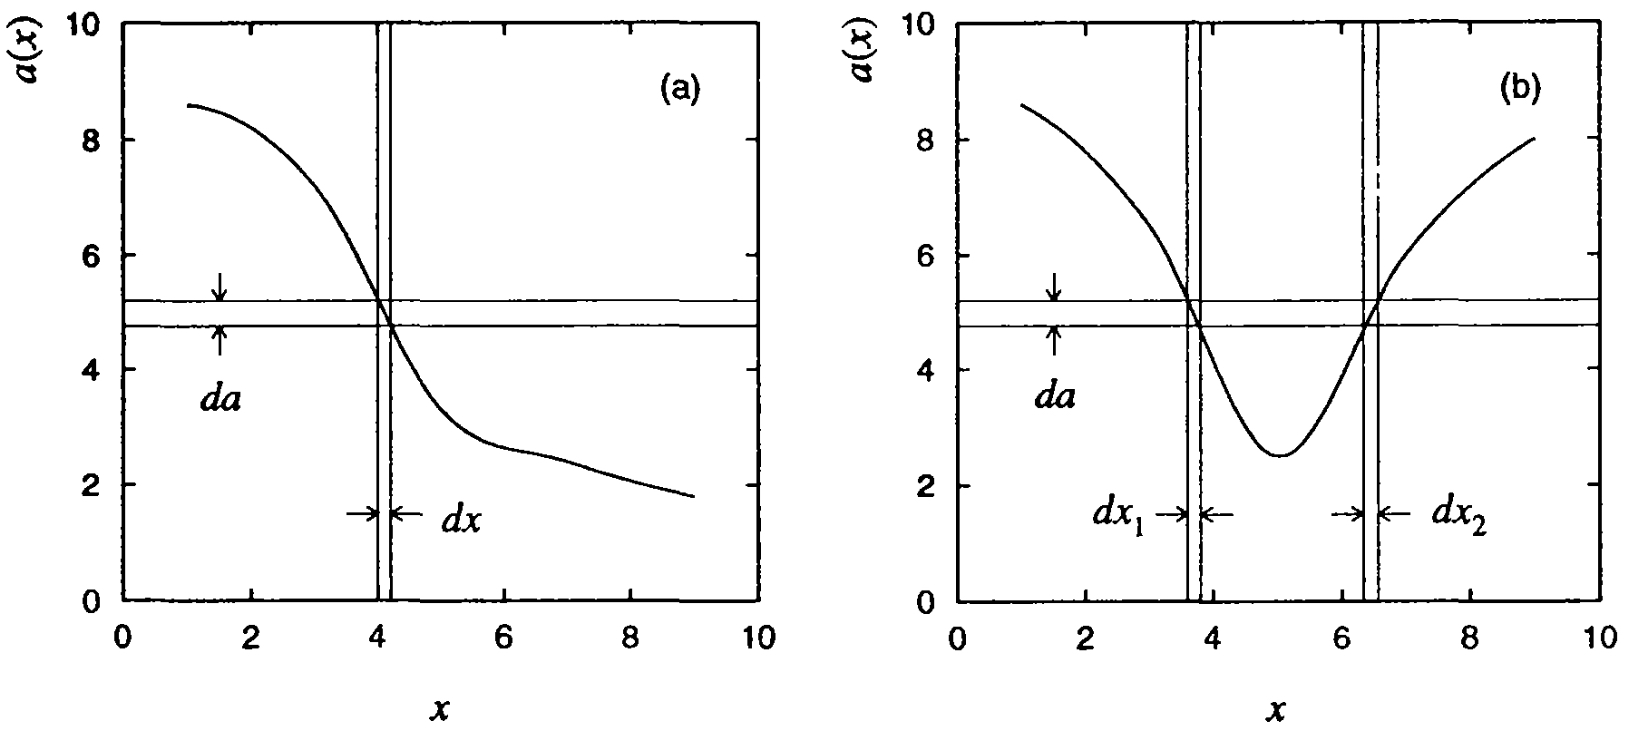
\includegraphics[width=0.65\textwidth,keepaspectratio]{RVfunc}
	\label{fig:RVfunc}
\end{figure}
%Distribuzione di probabilit\'a di $a(X)$ funzione di variabile casuale X con PDF $f(x)$:
\begin{align*}
%&g(a)=f(x(a))|\TDy{a}{x}|\tag*{g(a)\,da=f(x)\,dx}\\
&g(a)\,da=|\int_{x(a)}^{x(a+da)}f(x')\,dx'|=\int_{x(a)}^{x(a)+|\TDy{a}{x}|da}f(x')\,dx'\\
&\Rightarrow g(a)=f(x(a))|\TDy{a}{x}|\\
&g(a')d\,a'=\int_{dS=\{a'\leq a(\vec{x})\leq a'+d\,a'\}}f(x_1,\ldots,x_n)d^n\,x\\
&\prob{(y_1,\ldots,y_n)}=\frac{\prob{(x_1,\ldots,x_n)}}{|\left.\frac{\partial(y_1,\ldots,y_n)}{\partial(x_1,\ldots,x_n)}\right|_{x_1,\ldots,x_n=X_1(\vec{y}),\ldots,X_n(\vec{y})}|}\ (g(\vec{a})=f(\vec{x})|\underset{\PDy{\vec{a}}{\vec{x}}}{J}|)
\end{align*}
\end{frame}

\begin{wordonframe}{Somma e prodotto di 2 RV}
pdf di x \'e $g(x)$ e pdf di y \'e $h(y)$.
\begin{block}{Prodotto: $z=xy$}
	\begin{columns}[T]
		\begin{column}{0.3\textwidth}
			\begin{figure}
				\centering
				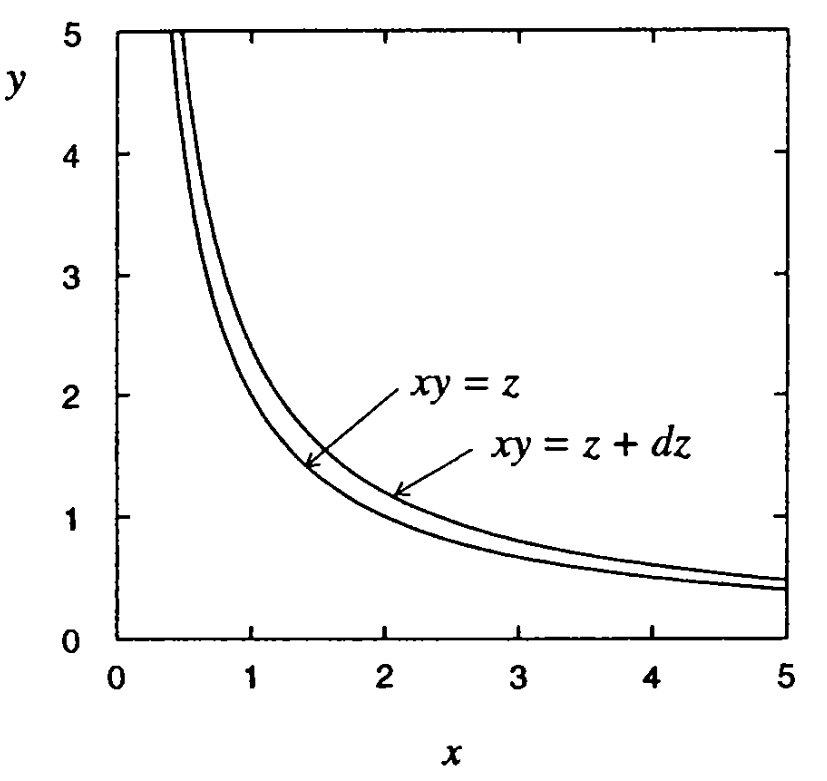
\includegraphics[keepaspectratio,width=0.9\textwidth]{RVprod}
				\label{fig:RVprod}
			\end{figure}
		\end{column}
		\begin{column}{0.7\textwidth}
			\begin{align*}
			&f(z)d\,z=\int_{d\,S}g(x)h(y)d\,xd\,y\\
			&=\intsinf{}g(x)d\,x\int_{\frac{z}{|x|}}^{\frac{z+d\,s}{|x|}}h(y)d\,y\\
			&f(z)=\intsinf{}g(\frac{z}{y})h(y)\frac{d\,y}{|y|}
			\end{align*}
		\end{column}
	\end{columns}
\end{block}
\begin{block}{Somma: $z=x+y$}
	\begin{align*}
	&f(z)=\intsinf{}g(x)h(z-x)d\,x=\intsinf{}g(z-y)h(y)d\,y
	\end{align*}
\end{block}
\end{wordonframe}

\begin{frame}{Sequenze di RV}\frameintoc
\begin{block}{Convergenza in distribuzione}
$\{X_n\}, X$ RV e $\{F_n\}, F$ cumulanti: $F_n\to F$
\end{block}
\begin{block}{Convergenza in probabilit\'a}
$\prob{(|X_n-X|>\epsilon)}\xrightarrow{n\to\infty}0$
\end{block}
\begin{block}{Teorema di Paul-Levy}
\begin{columns}[T]
	\begin{column}{0.3\textwidth}
		Se conosco tutti i momenti di una distribuzione conosco la distribuzione?
	\end{column}
	\begin{column}{0.7\textwidth}
		\begin{itemize}
			\item $F_n$ successione di funzioni cumulanti
			\item $\phi_n\to\phi$ per ogni $t\in I(0)$
			\item $\Re{\phi}$ continua in $I(0)$ (implica pdf \'e FT di $\phi$?)
		\end{itemize}
		quindi $F_n(x)\to F(x)$.
	\end{column}
\end{columns}
\end{block}
\begin{block}{Slutsky theorem}
$\{X_n\},\{Y_n\}$ sequence of scalar/vector RV: $\{X_n\}\xrightarrow{D}X,\{Y_n\}\xrightarrow{P}c$, quindi $\{X_n\}+\{Y_n\}\xrightarrow{D}X+c$, $\{X_nY_n\}\xrightarrow{D}c\{X_n\}$, $\{X_n/Y_n\}\xrightarrow{D}\{X_n/c\}$
\end{block}
\end{frame}

\begin{wordonframe}{Somma di 2 RV uniformi $U([0,1])$}
	\begin{columns}[T]
		\begin{column}{0.5\textwidth}
			\begin{align*}
			&S=x+y\\
			&\mu_1=\mu_2=\frac{1}{2}\\
			&\E{[S]}=\mu_1+\mu_2=1\\
			&\var{S}=\var{x}+\var{y}+2\cov{(x,y)}=\frac{1}{6}
			\end{align*}
			\noindent\rule{0.9\textwidth}{0.4pt}
		\end{column}
		\begin{column}{0.5\textwidth}
			\begin{align*}
			&z=x+y,\ z_2=y\\
			&J=\begin{pmatrix}
			\PDy{y_1}{x_1}(=1)&\PDy{y_1}{x_2}(=1)\\
			\PDy{y_2}{x_1}(=0)&\PDy{y_2}{x_2}(=1)\\
			\end{pmatrix}\\
			&\prob{(z,z_2)}=\frac{\prob_x{(z-z_2)}\prob_y{z_2}}{|\det{J}|}\\
			&\prob{(z)}=\left\{\begin{array}{c}
			\int_0^z\,dy\ (z<1)\\
			\int_{z-1}^1\ (z>1)\\
			0\ (z>2)\\
			\end{array}\right.\\
			&=\left\{\begin{array}{c}
			z\\
			2-z\\
			0\\
			\end{array}\right.\\
			&\E{[z]}=1,\ \var{[z]}=\frac{1}{6}
			\end{align*}
		\end{column}
	\end{columns}
\end{wordonframe}

\begin{wordonframe}{Prodotto di due RV $U([0,1])$}
	\begin{columns}[T]
		\begin{column}{0.5\textwidth}
			\begin{align*}
			&S=xy\\
			&\E{[S]}=\mu_x\mu_y\\
			&\var{[S]}=\mu_y^2\var{[x,x]}\\
			&+\mu_x^2\var{[y,y]}+2\mu_x\mu_y\var{[x,y]}\\
			&\E{[S]}=\frac{1}{4},\ \var{[S]}=\frac{1}{24}
			\end{align*}
		\end{column}
		\begin{column}{0.5\textwidth}
			\begin{align*}
			&z=xy,\ z_2=y,\ \det{J}=y\\
			&\prob{(z)}=\int_z^1\frac{\prob_x{(\frac{z}{y})}\prob_y{(y)}}{|y|}\,dy,\ 0\leq\frac{z}{y}\leq1\\
			&\prob{(z)}=\int_z^1\frac{1}{y}\,dy=\ln{\frac{1}{z}},\ (=0: z\notin[0,1])\\
			&\E{[z]}=\frac{1}{4},\ \var{[z]}=\num{0.0486}
			\end{align*}
		\end{column}
	\end{columns}
\end{wordonframe}

\begin{wordonframe}{Rapporto di due RV $U([0,1])$}
	\begin{columns}[t]
		\begin{column}{0.5\textwidth}
			\begin{align*}
			&S=\frac{x}{y},\ \E{[S]}=\frac{\mu_x}{\mu_y}=1\\
			&\var{(S)}=\frac{2}{3}\\
			&((\frac{\mu_x}{\mu_y})^2[\frac{\var{(x,x)}}{\mu_x^2}+\frac{\var_{xy}}{\mu_y^2}-\frac{2\cov_{xy}}{\mu_x\mu_y}])
			\end{align*}
			
			\noindent\rule{.9\textwidth}{0.1pt}\noindent
			
			\begin{picture}(100,130)
			\put(20,20){
				\begin{tikzpicture}[scale=0.55]
				%baseline=(current bounding box.south)
				\begin{axis}[ylabel={$y$},xlabel={$z$}]
				\addplot[color=green,fill=green,name path=one] function [raw gnuplot, id=rappmargp1, mark=none]{set xrange [0:1]; plot 1} node[right] {$1$};
				\addplot[color=green,name path=oneoverz] function [raw gnuplot, id=rapmargp2, mark=none]{set xrange [1:8]; plot 1/x} node[above right] {$\frac{1}{z}$};
				\path[name path=axisone] (axis cs:0,0) -- (axis cs:1,0);
				\path[name path=axistwo] (axis cs:1,0) -- (axis cs:8,0);
				\addplot[thick,color=blue, fill=blue, fill opacity=0.15] fill between[of=one and axisone];
				\addplot[thick,color=blue, fill=blue, fill opacity=0.15] fill between[of=oneoverz and axistwo];
				\end{axis}
				\end{tikzpicture}
			}
			\end{picture}
		\end{column}
		\begin{column}{0.4\textwidth}
			\begin{align*}
			&z=\frac{x}{y},\ z_2=y\\
			&\prob{(z,z_2)}=\frac{\prob_x{(zz_2)}\prob_y{z_2}}{|1/z_2|}\\
			&\prob{(z)}=\int\prob_x{(xy)}\prob_y{(y)}|y|\,dy\\
			&\prob{(z)}=\left\{\begin{matrix}\int_0^1y\,dy\ (z\leq1)\\\int_0^{1/z}y\,dy=\frac{1}{2z^2}\ (z\geq1)\\0\ (z<0)\end{matrix}\right.
			\end{align*}
			\keyword{EX: Rapporto RV uniformi}
		\end{column}
	\end{columns}
\end{wordonframe}

\begin{wordonframe}{Rapporto di gaussiane}
	\begin{columns}[T]
		\begin{column}{0.5\textwidth}
			\begin{align*}
			&x=G{(0,1)},\ y=G{(0,1)},\ z=\frac{x}{y}\\
			&\prob{(z)}=\frac{1}{2\pi}\intsinf{}dy\,\exp{-\frac{(zy)^2}{2}}|y|\\
			&=\frac{1}{\pi}\intzi{}\,dy\exp{-\frac{y^2}{2}(1+z^2)}
			\end{align*}
		\end{column}
		\begin{column}{0.5\textwidth}
			\begin{align*}
			&u=y\sqrt{1+z^2}:\\
			&\prob{(z)}=\frac{1}{\pi}\frac{1}{1+z^2}\intzi{}du\,u\exp{-\frac{u^2}{2}}
			\end{align*}
		\end{column}
	\end{columns}
	$\prob{(z)}$ \'e proporzionale a Cauchy:
	\begin{align*}
	&\E{(z^2n)}=\infty\\
	&\E{(z^{2n+1})}=Ind
	\end{align*}
	\begin{block}{\keyword{Somma di Cauchy}: $S=x+y$}
		\[\prob{(S)}=\int_{-\infty}^{+\infty}\frac{1}{\pi}\frac{1}{1+x^2}\frac{1}{\pi}\frac{1}{1+(S-X)^2}\,dx\to\frac{1}{2\pi}\frac{1}{1+(\frac{S}{2})^2}\]
	\end{block}
\end{wordonframe}

\begin{frame}[allowframebreaks]{Esempi probabilit\'a condizionata: double layered detector, dadi Dungeons\& Dragon, ammo}
\begin{block}{Double layered detector}
	\begin{columns}[T]
		\begin{column}{0.5\textwidth}
			Detector a due strati attraversato da fascio di particelle (\num{e-4} elettroni e il resto fotoni); la probabilit\'a di un segnale in zero, uno o entrambi gli strati \'e:
			\begin{align*}
			&\prob{(0|e)}=0.001,\ \prob{(0|\gamma)}=0.99899\\
			&\prob{(1|e)}=0.01\ \prob{(0|\gamma)}=0.001\\
			&\prob{(2|e)}=0.989\ \prob{(0|\gamma)}=\num{e-5}\\
			\end{align*}
		\end{column}
		\begin{column}{0.5\textwidth}
			Probabilit\'a che particella rivelata in solo uno strato sia fotone:
			\begin{align*}
			&\prob{(\gamma|1)}=\frac{\prob{(1|\gamma)}\prob{(\gamma)}}{\prob{(1)}}\\
			&=\frac{\num{e-3}(1-\num{e-4})}{\num{e-2}(1-\num{e-4})+\num{e-2}\num{e-4}}\\
			&(\prob{(1)}=\prob{(1|e)}\prob{(e)}+\prob{(1|\gamma)}\prob{(\gamma)})\\
			&\prob{(0)}\approx 1,\ \prob{(1)}\approx\num{e-3},\ \prob{(2)}\approx\num{e-4}
			\end{align*}
		\end{column}
	\end{columns}
\end{block}
\framebreak
\begin{block}{Dadi Dungeons\& Dragons}
	Sei dadi $D_i$ con numero di facce $i=\{4,6,8,10,12,20\}$.
	\begin{align*}
	&\prob{(1)}=\sum\prob{(1|D_i)}\prob{(D_i)}=\sum_i\frac{1}{i}\frac{1}{6}\approx0.129\intu{\keyword{T. probabilit\'a totale}}\\
	&\prob{(D_i|1)}=\frac{\prob{(1|D_i)\prob{(D_i)}}}{\prob{(1)}}=\frac{\frac{1}{i}\frac{1}{6}}{\frac{1}{6}\sum\frac{1}{i}}\\
	&\prob{(1|1)}=\sum_i\prob{(1|D_i,1)}\prob{(D_i|1)}&\intertext{(indipendenti: $\prob{(A|B)}=\prob{(A)}$)}
	&=\sum\frac{1}{i}\prob{(D_i|1)}=\sum\frac{1/i^2}{\sum1/i}\approx0.161\\
	&(\prob{(D_i|1)}=\frac{\prob{(1|D_i)}\prob{(D_i)}}{\prob{(1)}})
	\end{align*}
\end{block}
\begin{block}{Casse di munizioni}
	Dopo tempo T in deposito delle casse di munizioni hanno nel $90\%$ dei casi una frazione di proiettili danneggiati $f_D=0=q$, nel $10\%$ dei casi $f_D=0.05=q$ ($\prob{(q)}=0.9\delta(q)+0.1\delta(q-0.05)$). Quante munizioni devo testare per cassa e con quale $f_D$ per avere percentuale casse danneggiate minore del $5\%$?
	\begin{align*}
	&\prob{(q|k)}=\frac{\prob{(k|q)}\prob{q}}{\prob{k}}\\
	&\prob{(k|q)}=\binom{n}{k}q^k(1-q)^{n-k}\\
	&\prob{(q|k)}=\frac{\binom{n}{k}q^k(1-q)^{n-k}[0.9\delta(q)+0.1\delta(q-0.05)]}{\int\,dq\binom{n}{k}q^k(1-q)^{n-k}[0.9\delta(q)+0.1\delta(q-0.05)]}\\
	&\prob{(q=0|k=0)}\geq0.96,\ n=20
	\end{align*}
\end{block}
\end{frame}

\subsection{Propagazione errori}

\begin{frame}{Propagazione errori}
\begin{align*}
&S(\vec{x})\approx y(\vec{\mu})+\left.\sum_i^n\PDy{x_i}{S}\right|_{\vec{\mu}}(x_i-\mu_i)+o(|\vec{x}-\vec{\mu}|)\\
&\var{(S)}=\E{[(S(\vec{x})-\E{[S]})^2]}\approx\sum_{ij}\PDyat{x_i}{S}{\vec{\mu}}\PDyat{x_i}{y}{\vec{\mu}}\cov{x_ix_j}
\end{align*}
\begin{block}{Covarianza e correlazione}
\begin{columns}[T]
\begin{column}{0.5\textwidth}
\begin{align*}
&\cov{x_ix_j}=\E{[(x-\mu_x)(y-\mu_y)]}=\E{[xy]}-\mu_x\mu_y
\end{align*}
\end{column}
\begin{column}{0.5\textwidth}
\begin{align*}
\rho_{xy}=\frac{\cov{x_ix_j}}{\sigma_i\sigma_j}
\end{align*}
\end{column}
\end{columns}
X,Y indipendenti: $\rho_{XY}=0$ ma non v.v.
\end{block}
\end{frame}

\subsection{Funzione caratteristica}\linkdest{moments}

\begin{frame}{Funzione generatrice dei momenti - Funzione caratteristica}
\begin{columns}[T]
	\begin{column}{0.5\textwidth}
		\begin{align*}
		&M_X(t)=\E{[\exp{tX}]}\\
		&\phi_X(t)=\E{[\exp{itX}]}=\int\exp{itx}\,d\mu_X(x)\\
		&\phi(0)=1,\ |\phi(t)|\leq1\\
		&\phi_X(t)=1+i\mu t+\frac{1}{2}(\sigma^2+\mu^2)(it)^2
		\end{align*}
		\begin{block}{Somma RV (indipendenti))}
			\begin{align*}
			&X=X_1+X_2\\
			&M_X(t)=M_{X_1}M_{X_2}\\
			&(f(Z=X+Y)=\intsinf{}f_X(Z-t)f_Y(t)\,dt)
			\end{align*}
		\end{block}
	\end{column}
	\begin{column}{0.5\textwidth}
		\begin{align*}
		&\PDyn{t}{M_X}{n}|_{t=0}=\E{[x^n]}=\mu_n'\\
		&\PDyn{(it)}{\phi_X}{n}|_{t=0}=\left.(-i)^n\E{[x^n]}\right|_{t=0}=\mu_n'\\
		&\phi_X(t)=\E{[\sum_r\frac{(itX)^r}{r!}]}\\
		&=\sum_r\frac{(it)^r}{r!}\E{[X^r]}=\sum_r\frac{(it)^r}{r!}\mu_r'
		\end{align*}
		\begin{block}{Trasf lineare}
			\begin{align*}
			&Y=\alpha X+b\\
			&M_Y=\exp{ibt}M_X(\alpha t)
			\end{align*}
		\end{block}
	\end{column}
\end{columns}
Determina completamente pdf: se $F(X)$ continua, $dF(X)=f(X)dX$ allora $f(X)=\frac{1}{2\pi}\intsinf{}\phi_X(t)\exp{-iXt}\,dt$.
\end{frame}

\begin{frame}{Momenti di una distribuzione e di una statistica}
%Valore di aspettazione, varianza e momenti di di variabile casuale con data distribuzione di probabilit\'a, di campione (misure) estratto con data pdf e statistiche.
\begin{block}{Valore di aspettazione}
\begin{align*}
&E[X]=(\sum x_iP(X=x_i))=\int f(x)x\,dx\\
&E[a(X)]=\intsinf{}a(x)f(x)\,dx=\intsinf{}ag(a)d\,a
\end{align*}
Non \'e detto che $f(\mu)=\E{[f]}$.
\end{block}
\begin{columns}[T]
\begin{column}{0.6\textwidth}
\begin{block}{Varianza}
\begin{align*}
&\var{(x_n)}=E[(x_n-\mu)^2]=\mu_2=\sigma^2(X)
\end{align*}
\end{block}
\end{column}
\begin{column}{0.4\textwidth}
\begin{block}{Momenti successivi}
\begin{align*}
&\mu_l=E[(X-\mu)^l]
\end{align*}
\end{block}
\end{column}
\end{columns}
\begin{columns}[T]
\begin{column}{0.45\textwidth}
\begin{block}{Momenti di una statistica S}
\begin{align*}
    &\E{[(S(\vec{x})-\E{[S]})^l]}
\end{align*}
\end{block}
\end{column}
\begin{column}{0.55\textwidth}
\begin{block}{Relazione tra $\mu_n$ e $\mu'_n$.}
\begin{align*}
&\mu_n(x_0)=\E{[(X-\mu)^n]}=\sum_k^n\binom{n}{k}(-1)^{n-k}\mu'_kx_0^{n-k}
\end{align*}
\end{block}
\end{column}
\end{columns}
\end{frame}

\begin{wordonframe}{FGM pdf uniforme}
\begin{columns}[T]
\begin{column}{0.5\textwidth}
\begin{align*}
&p(x)=\frac{1}{m}\ 0<x<m\ (\int_0^mp(x)d\,x=1)\\
&\E{[\exp{tx}]}=\int_0^m\frac{\exp{tx}}{m}d\,x=\frac{\exp{mt}-1}{mt}\\
&=\frac{1}{m}[m+\frac{m^2t}{2}+\frac{m^3t^2}{6}+\frac{m^4t^3}{4!}+\ldots]
\end{align*}
\end{column}
\begin{column}{0.5\textwidth}
\begin{align*}
&\mu'_2=\frac{m^2}{3}=\sigma^2+\mu^2\\
&\sigma^2=\mu_2'-(\frac{m^2}{2})^2=\frac{m^2}{12}
\end{align*}
\end{column}
\end{columns}
\begin{block}{Somma RV con pdf uniforme fra 0 e 1}
$y=x_1+\ldots+x_n$: $\MGF_y=(\frac{\exp{mt}-1}{mt})^n$
\end{block}
\end{wordonframe}

\begin{wordonframe}{(contro)Esempi momenti}
\begin{block}{pdf di \keyword{Cauchy}: non vale LLN}
\keyword{Parametri larghezza e posizione}: $\prob{(x)}=\frac{1}{\pi\Gamma}\frac{1}{1+(\frac{x-m}{\Gamma})^2}$.
\begin{columns}[T]
\begin{column}{0.5\textwidth}
\begin{align*}
&\mu_1=\frac{1}{\pi}\intsinf{}\frac{x}{1+x^2}=\NAN{}\\
&\phi_c(t)=\intsinf{}\frac{\exp{ixt}}{\pi(1+x^2)}=\exp{-|t|}\\
&\phi_{\frac{X_1+X_2}{2}}=\exp{-|t|}
\end{align*}
\end{column}
\begin{column}{0.5\textwidth}
\begin{align*}
&F(x)=\intsinf{}\frac{1}{\pi}\frac{1}{1+x^2}d\,x=\frac{\arctan{x}}{\pi}+\frac{1}{2}
\end{align*}
\end{column}
\end{columns}
Per gaussiana: $\phi_{\overline{X}}(t)=\exp{-\frac{t^2}{4}}$, $\sigma^2\to\frac{\sigma^2}{2}$.
\end{block}
\end{wordonframe}

\begin{frame}{Funzione generatrice dei momenti - Funzione caratteristica}
\begin{columns}[T]
\begin{column}{0.5\textwidth}
\begin{align*}
&M_X(t)=\E{[\exp{tX}]}\\
&\phi_X(t)=\E{[\exp{itX}]}=\int\exp{itx}\,d\mu_X(x)\\
&\phi(0)=1,\ |\phi(t)|\leq1\\
&\phi_X(t)=1+i\mu t+\frac{1}{2}(\sigma^2+\mu^2)(it)^2
\end{align*}
\begin{block}{Somma RV (indipendenti))}
\begin{align*}
&X=X_1+X_2\\
&M_X(t)=M_{X_1}M_{X_2}\\
&(f(Z=X+Y)=\intsinf{}f_X(Z-t)f_Y(t)\,dt)
\end{align*}
\end{block}
\end{column}
\begin{column}{0.5\textwidth}
\begin{align*}
&\PDyn{t}{M_X}{n}|_{t=0}=\E{[x^n]}=\mu_n'\\
&\PDyn{it}{\phi_X}{n}|_{t=0}=\left.(-i)^n\E{[x^n]}\right|_{t=0}=\mu_n'\\
&\phi_X(t)=\E{[\sum_r\frac{(itX)^r}{r!}]}\\
&=\sum_r\frac{(it)^r}{r!}\E{[X^r]}=\sum_r\frac{(it)^r}{r!}\mu_r'
\end{align*}
\begin{block}{Trasf lineare}
\begin{align*}
&Y=\alpha X+b\\
&M_Y=\exp{ibt}M_X(\alpha t)
\end{align*}
\end{block}
\end{column}
\end{columns}
Determina completamente pdf: se $F(X)$ continua, $dF(X)=f(X)dX$ allora $f(X)=\frac{1}{2\pi}\intsinf{}\phi_X(t)\exp{-iXt}\,dt$.
\end{frame}

\begin{wordonframe}{FGM pdf uniforme}
\begin{columns}[T]
\begin{column}{0.5\textwidth}
\begin{align*}
&p(x)=\frac{1}{m}\ 0<x<m\ (\int_0^mp(x)d\,x=1)\\
&\E{[\exp{tx}]}=\int_0^m\frac{\exp{tx}}{m}d\,x=\frac{\exp{mt}-1}{mt}\\
&=\frac{1}{m}[m+\frac{m^2t}{2}+\frac{m^3t^2}{6}+\frac{m^4t^3}{4!}+\ldots]
\end{align*}
\end{column}
\begin{column}{0.5\textwidth}
\begin{align*}
&\mu'_2=\frac{m^2}{3}=\sigma^2+\mu^2\\
&\sigma^2=\mu_2'-(\frac{m^2}{2})^2=\frac{m^2}{12}
\end{align*}
\end{column}
\end{columns}
\begin{block}{Somma RV con pdf uniforme fra 0 e 1}
$y=x_1+\ldots+x_n$: $\MGF_y=(\frac{\exp{mt}-1}{mt})^n$
\end{block}
\end{wordonframe}

\begin{frame}{Teorema di Paul-Levy}
	\begin{columns}[T]
		\begin{column}{0.3\textwidth}
			Se conosco tutti i momenti di una distribuzione conosco la distribuzione?
		\end{column}
		\begin{column}{0.7\textwidth}
			\begin{itemize}
				\item $F_n$ successione di funzioni cumulanti
				\item $\phi_n\to\phi$ per ogni $t\in I(0)$
				\item $\Re{\phi}$ continua in $I(0)$ (implica pdf \'e FT di $\phi$?)
			\end{itemize}
			quindi $F_n(x)\to F(x)$.
		\end{column}
	\end{columns}
\end{frame}

\begin{wordonframe}{Funzioni caratteristiche}
\begin{columns}[T]
	\begin{column}{0.5\textwidth}
Gaussiana: $\phi_X(t)=\exp{\mu it-\frac{\sigma^2t^2}{2}}$
	\end{column}
	\begin{column}{0.5\textwidth}
Poissoniana: $\Phi_X(t)=\exp{\lambda(\exp{it}-1)}$
	\end{column}
\end{columns}
\end{wordonframe}

\section{Math tools}\linkdest{math}

\begin{wordonframe}{Taylor and others}
$(a+b)^n=\sum_{k=0}^n\binom{n}{k}a^{n-k}b^k$
\end{wordonframe}

\begin{wordonframe}{Propriet\'a Trasformata di Fourier}
\begin{columns}
\begin{column}{0.5\textwidth}
\begin{align*}
f(x)\FT{}\begin{matrix}
\hat{f}(\omega)=\frac{1}{\sqrt{2\pi}}\intsinf\,f(x)\exp{-i\omega x}\,dx\\
\hat{f}(\nu)=\intsinf\,f(x)\exp{-i\nu x}\,dx\\
\end{matrix}
\end{align*}
\end{column}

\begin{column}{0.5\textwidth}
\begin{align*}
&a*f(x)+bg(x)\FT{}a\hat{f}(\nu)+b\hat{g}(\nu)\\
&h(x)=\exp{2\pi ix\nu_0}f(x)\FT{}\hat{f}(\nu-\nu_0)
\end{align*}
\end{column}
\end{columns}

\begin{columns}
\begin{column}{0.5\textwidth}
Scalar: \[f(ax)\FT{}\frac{1}{|a|}\hat{f}(\frac{\omega}{a}) \]
Translations:
\[f(x-a)\FT{}\exp{-ia\nu}\hat{f}(\nu)f(x)\exp{iax}\]
\[\hat{f}(\xi-\frac{a}{2\pi}) \hat{f}(\nu-a)\]

Derivates:
\[\frac{d^n\,f(x)}{dx^n}\FT{}(i\omega)^n\hat{f}(\omega)\]
\[x^nf(x)\FT{}i^n\frac{d^n\hat{f}(\omega)}{d\omega^n}\]
\end{column}
\begin{column}{0.5\textwidth}
Inverse: \[\hat{a} f(-\omega) 2\pi f(-\nu)\]
Convoluzione e prodotto:
\begin{align*}
&(f*g)(x)\FT{}\sqrt{2\pi}\hat{f}(\omega)\hat{g}(\omega)\\
&\hat{f}(\nu)\hat{g}(\nu)\\
&f(x)g(x)\FT{}\frac{1}{\sqrt{2\pi}}(\hat{f}*\hat{g})(\omega)\\
&\FT{}\frac{1}{2\pi}(\hat{f}*\hat{g})(\nu)
\end{align*}

\end{column}
\end{columns}
\end{wordonframe}

\begin{wordonframe}{Trasformata di Fourier notevoli}
\begin{align*}
& 1 & \sqrt{2\pi}\delta(\omega) & 2\pi\delta(\nu)\delta(x)\\
& \delta(x) & \frac{1}{\sqrt{2\pi}} & 1\\
& \exp{iax} & \sqrt{2\pi}\delta(\omega-a) & 2\pi\delta(\nu-a)\\
& x^n & i^n\sqrt{2\pi}\delta^{(n)}(\omega) & 2\pi i^n\delta^{(n)}(\nu)\\
& \frac{1}{x^n} & -i\sqrt{\frac{\pi}{2}}\frac{(-i\omega)^{n-1}}{(n-1)!}\sgn{(\omega)} & -i\pi\frac{(-i\nu)^{n-1}}{(n-1)!}\sgn{(\nu)}\\
& |x|^{\alpha} & \frac{-2}{\sqrt{2\pi}}\frac{\sin{(\frac{\pi\alpha}{2})}\Gamma(\alpha+1)}{|\omega|^{\alpha+1}} & -2\frac{\sin{(\frac{\pi\alpha}{2})}\Gamma(\alpha+1)}{|\nu|^{\alpha+1}}\\
& \frac{1}{\sqrt{|x|}} & \frac{1}{\sqrt{|\omega|}} & \sqrt{\frac{2\pi}{\nu}}\\
& \sgn{x} & \sqrt{\frac{2}{\pi}}\frac{1}{i\omega} & \frac{2}{i\nu}\\
& \rect{(ax)} & \frac{1}{\sqrt{2\pi a^2}}\sinc{(\frac{\omega}{2\pi a})} &  \frac{1}{|a|}\sinc{(\frac{\nu}{2\pi a})}\sinc{(ax)}\\
\end{align*}

\end{wordonframe}

\begin{wordonframe}{Trasformata di Fourier notevoli II}

\begin{align*}
&\sinc{(ax)} & \frac{1}{\sqrt{2\pi a^2}}\rect{(\frac{\omega}{2\pi a})} &  \frac{1}{|a|}\rect{(\frac{\nu}{2\pi a})}\\
&\sinc^2{(ax)} & \frac{1}{\sqrt{2\pi a^2}}\tri{(\frac{\omega}{2\pi a})} &  \frac{1}{|a|}\tri{(\frac{\nu}{2\pi a})}\\
&\tri{(ax)} & \frac{1}{\sqrt{2\pi a^2}}\sinc^2{(\frac{\omega}{2\pi a})} &  \frac{1}{|a|}\sinc^2{(\frac{\nu}{2\pi a})}\\
&\exp{-\alpha x^2} & \frac{1}{\sqrt{2\alpha}}\exp{-\frac{\omega^2}{4\alpha}} & \sqrt{\frac{\pi}{\alpha}}\exp{-\frac{\nu^2}{4\alpha}}\\
&\exp{-a|x|} & \sqrt{\frac{2}{\pi}}\frac{a}{a^2+\omega^2} & \frac{2a}{a^2+\nu^2}\exp{-\frac{a^2x^2}{2}}\\
&\exp{-\frac{a^2x^2}{2}}H_n(ax) & \frac{(-i)^n}{a}\exp{-\frac{\omega^2}{2a^2}}H_n(\frac{\omega}{a}) & \frac{(-i)^n\sqrt{2\pi}}{a}\exp{-\frac{\omega^2}{2a^2}}H_n(\frac{\nu}{a})\\
&\exp{-a|x|} & \frac{2a}{x^2+a^2}
\end{align*}
\end{wordonframe}

\section{Legge grandi numeri - Teorema limite centrale}\linkdest{lln-clt}

\begin{frame}{Legge grandi numeri}
$X_1,\ldots,X_n$ iid RV (RV campionata n volte): $\E{X_i}=\mu$, finite variance: $\var{X_i}=\sigma^2$ allora \[\prob{(|\overline{X}_n-\mu|>\epsilon)}\leq\frac{\sigma^2}{n\epsilon^2}\]
    \begin{columns}
    \begin{column}{0.4\textwidth}
\begin{align*}
&\var{\overline{X}_n}=\var{\frac{1}{n}(X_1+\ldots+X_n)}\\
&=\frac{1}{n^2}\var{(X_1+\ldots+X_n)}\\
&=\frac{n\sigma^2}{n^2}=\frac{\sigma^2}{n}\\
&\prob{(|\overline{X}_n-\mu|>\epsilon)}\leq\frac{\sigma^2}{n\epsilon^2}
\end{align*}
    \end{column}
    \begin{column}{0.6\textwidth}
Per ogni RV con $\mu$ finita $\phi_X(t)\approx1+i\mu t+o(t)$,$\phi_{\frac{1}{n}X}(t)=\phi_X(\frac{t}{n})$, $\phi_{X+Y}(t)=\phi_X(t)\phi_Y(t)$:
$\phi_{\overline{X}_n}(t)=[\phi_X(t)]^n=[1+it\mu+\ldots]^n\to\exp{i\mu t}$; Levy theorem: $\overline{X}_n\to\mu$.
\keyword{Chebyshev ineq}: $\prob{(|X-\mu|\geq k\sigma)}\leq\frac{1}{k^2}$.
\keyword{Probability convergence}: Una sequenza di RV $\{X_n\}\to X$ in probabilit\'a se $\lim_{n\to\infty}\prob{(|X_n-X|)>\epsilon}$=0.
    \end{column}
    \end{columns}
\end{frame}

\begin{frame}{LLN: asintoticamente gaussiana - Teorema limite centrale (CLT)}
Se esistono $\mu_1, \mu_2$ finiti vale LLN: $\overline{x}_n-\mu\xrightarrow{P}0$.
\begin{columns}[T]
\begin{column}{0.5\textwidth}
\begin{align*}
&\var{(\overline{x}_n-\mu)}=\var{(\frac{S_N}{N})}\\
&=\frac{1}{N^2}\var{(S_N)}=\frac{\sigma^2}{N}\\
&\var{(S_N)}=\sum(\PDy{x_i}{S_N})^2\sigma_i^2
%&\phi(t)=\phi_{X-\mu}
\end{align*}
\end{column}
\begin{column}{0.5\textwidth}
\begin{align*}
&y_N=\sqrt{\frac{N}{\sigma^2}}(\overline{x}-\mu)\\
&\E{[y_N]}=0,\ \var{[y_N]}=1\\
&\phi_N=[\phi(\frac{t}{\sigma\sqrt{N}})]^N
\end{align*}
\end{column}
\end{columns}
\[\phi(t)=\sum_{m=0}^{\infty}\left.\frac{d^m\phi}{dt^m}\right|_{t=0}\frac{t^m}{m!}=\sum_{m=0}^{\infty}\frac{(it)^m}{m!}\E{(y^m)}\approx1-\frac{t^2}{2N}\sigma^2-\frac{it^3}{3!}\frac{\E{[(x-\mu)^3]}}{n\expy{3/2}}+\ldots\]
\begin{align*}
&\log{\phi_N}=N\log{\phi(\frac{t}{\sigma\sqrt{N}})}\approx N[\frac{it\mu}{\sigma\sqrt{N}}+\frac{(it)^2\sigma^2}{2\sigma N}+o(\frac{t^3}{N\expy{\frac{3}{2}}})]\to-\frac{t^2}{2}\\
%\text{Per T Levy la pdf \'e:}\\
&\frac{1}{2\pi}\int\exp{-\frac{t^2}{2}}\exp{-itx}d\,t=\frac{1}{2\pi}\int\exp{(t+ix)^2-\frac{x^2}{2}}\,dt=\frac{\exp{-\frac{x^2}{2}}}{\sqrt{2\pi}}
\end{align*}
\end{frame}

\begin{wordonframe}{Espansioni di Taylor}
\begin{align*}
&\phi(t)=1+it\mu-\frac{\sigma^2t^2}{2}+o(t^2)\\
&\log{(1+x)}\approx x-\frac{x^2}{2}+o(x^2)
\end{align*}
\end{wordonframe}

\begin{frame}{Examples where CLT breaks down}
\begin{itemize}
\item Total number of electron-ion pair created when charged particle traverses matter: Landau distribution.
\item Angle by which a charged particle is deflected traversing matter
\end{itemize}
\end{frame}

\section{Important pdfs}\linkdest{pdfs}

\begin{wordonframe}{Combinazioni e permutazioni}
\begin{itemize}
\item $n!$: permutazioni - modi distinti di prendere n oggetti
\item Permutazioni senza ripetizioni - Arrengements of n objects taken k at a time: $P_{nk}=\frac{n!}{(n-k)!}$.
\item Combinazioni senza ripetizioni $C_{nk}=\frac{n!}{k!(n-k)!}$
\end{itemize}
\end{wordonframe}

\begin{frame}{Gaussian}
\begin{columns}[T]
\begin{column}{0.5\textwidth}
\begin{align*}
&\prob{[x]}=f(x)=\frac{1}{\sqrt{2\pi}\sigma}\exp{-\frac{(x-\mu)^2}{2\sigma^2}}\\
&F(x)=\frac{1}{2}[1+\Erf([\frac{x-\mu}{\sqrt{2}\sigma}])
\end{align*}
\end{column}
\begin{column}{0.5\textwidth}
\begin{align*}
\phi_X(t)=\exp{\mu it-\sigma^2\frac{t^2}{2}}
\end{align*}
\end{column}
\end{columns}
\todo{Somma N gaussiane?}
\end{frame}

\begin{frame}{Bernoulli, binomiale}
\begin{block}{Bernoulli: 2 possibili outcomes}
	\begin{columns}[T]
	\begin{column}{0.5\textwidth}
	\begin{align*}
	&\prob{(X=1)}=p=1-\prob{(X=0)}=1-q
	\end{align*}
	\end{column}
	\begin{column}{0.5\textwidth}
	\begin{align*}
	&\E{X}=p,\ \var{X}=qp\\
	&CF: q+p\exp{it}
	\end{align*}
	\end{column}
	\end{columns}
\end{block}
\begin{block}{Distribuzione binomiale: k eventi con probabilit\'a p in sequenza di n estrazioni. Somma n variabili Bernoulli.}
\begin{align*}
&\prob{(k;n,p)}=\binom{n}{k}p^k(1-p)^{n-k}
\end{align*}
\begin{align*}
&\E{[k]}=\sum_kk\frac{N!}{k!(N-k)!}p^k(1-p)\expy{N-k}=Np\\
&\mu'_q=\sum_k^nk^q\binom{n}{k}p^k(1-p)^{n-k}\\
&M_X(t)=\E{[\exp{tX}]}=\sum_k\exp{tk}\binom{n}{k}p^k(1-p)^{n-k}=M_B^n(t)
\end{align*}
\end{block}
\end{frame}

\begin{frame}{Multinomiale: n trials with one success between k categories}
	\begin{align*}
	&f(x_1,\ldots,x_k;n,p_1,\ldots,p_k)=\frac{n!}{x_1!\ldots x_k!}p_1\expy{x_1}\ldots p_k\expy{x_k}:\ \E{[X_i]}=Np_i\\
	&\var{[X_i]}=Np_i(1-p_i)\\
	&CF: (\sum_j^kp_j\exp{it_j})^n
	\end{align*}
\end{frame}

\begin{wordonframe}{Derivazione pdf Bernoulli}
\begin{columns}[T]
\begin{column}{0.3\textwidth}
\begin{block}{Bernoulli}
\begin{align*}
&\underbrace{0110010}_{n:k(1)\leq n}0110\ldots\\
&\prob{(1)}=\lim_{N\to\infty}\frac{\#(1's)}{N}\\
&\prob{(0)}=1-\prob{(1)}\\
\end{align*}
\noindent\rule{0.9\textwidth}{0.4pt}
\end{block}
\end{column}
\begin{column}{0.7\textwidth}
\begin{block}{Binomiale}
\begin{align*}
&\prob{(k;n,p)}\ \text{Ensamble di N sottosequenze}\\
&\prob{(1\ldots);n,p}=\lim_{N\to\infty}(\frac{\#\overbrace{(1\ldots)}^n}{N})=p\\
&\prob{(11\ldots);n,p}=\lim_{N\to\infty}(\frac{\#\overbrace{(11\ldots)}^n}{N})\\
&=\lim_{N\to\infty}\frac{n(1\ldots)}{N}\frac{n(11\ldots)}{n(1\ldots)}=p^2, \ldots
\end{align*}
\end{block}
\end{column}
\end{columns}
\begin{align*}
&\prob{(\overbrace{(1,\ldots,1}^k,\underbrace{0,\ldots,0})}_{n-k})=p^k(1-p)^{n-k}
\end{align*}
\begin{columns}[T]
\begin{column}{0.2\textwidth}
\begin{align*}
&\binom{n}{k}=\frac{n!}{k!(n-k)!}
\end{align*}
\end{column}
\begin{column}{0.8\textwidth}
fattore binomiale che tiene conto delle permutazioni di n elementi e del fatto che $k$ e $(n-k)$ sono identici.
\end{column}
\end{columns}
\end{wordonframe}

\begin{wordonframe}{Calcolo MGF per binomiale}
\begin{columns}[T]
\begin{column}{0.5\textwidth}
\begin{block}{Somma di n Bernoulli}
\begin{align*}
&X=X_1+\ldots X_n\\
&M_B(t)=E_B[\exp{tX}]\\
&=(1-p)\exp{0}+\exp{t}p
\end{align*}
\end{block}
\end{column}
\begin{column}{0.5\textwidth}
\begin{block}{Explicit method}
\begin{align*}
&\sum_k^n\binom{n}{k}(\exp{t}p)^k(1-p)^{n-k}\\
&(a+b)^n=\sum_k\binom{n}{k}a^kb^{n-k}
\end{align*}
\end{block}
\end{column}
\end{columns}
\begin{align*}
&M_k=[(1-p)+p\exp{t}]^n
\end{align*}
\end{wordonframe}

\begin{frame}{Poissoniane!}
\begin{columns}[T]
	\begin{column}{0.5\textwidth}
\[\prob{(k;n,p)}=\binom{n}{k}p^k(1-p)^{n-k}\]
Nel limite piccolo $p=c\Delta t=\frac{\lambda T}{n}$:
\begin{align*}
&\underbrace{[\frac{n}{n}\ldots\frac{n-k+1}{n}]}_{1}\frac{1}{k!}[\frac{\lambda T}{1-\frac{\lambda T}{n}}]^k(1-\frac{\lambda T}{n})^n\\
&\to\frac{(\lambda T)^k}{k!}\exp{-\lambda T}\\
&\prob{(x\leq k)}=\frac{\Gamma(\lfloor k+1\rfloor,\lambda)}{\lfloor k\rfloor}=\exp{-\lambda}\sum_{i=0}^k\frac{\lambda^i}{i!}
\end{align*}
	\end{column}
	\begin{column}{0.5\textwidth}
		\begin{align*}
&\prob{(k;\mu)}=\frac{\mu^k}{k!}\exp{-\mu}\\
&\prob{(r<N_0|\mu)}\\
&=1-\prob{(\chi^2_{2N_0+2}<2\mu)}\\
&\E{[k]}=\sum_{k=0}^{\infty}k\frac{\mu^k}{k!}\exp{-\mu}\\
&\E{[k^2]}=\sum_{k=0}^{\infty}k^2\frac{\mu^k}{k!}\exp{-\mu}=\mu^2+\mu\\
&\var[k]=\E{[k^2]}-(\E{[k]})^2=\mu
\end{align*}
	\end{column}
\end{columns}
\begin{align*}
&M_P(t)=\sum_k\exp{tk}\frac{\mu^k}{k!}\exp{-\mu}=\Exp{\mu(\exp{t}-1)}
\end{align*}
\todo{Ex: media e varianza Poissoniana}
\todo{Somma di N Poissoniane}
\end{frame}

\begin{frame}{Irwin-Hall}
$X=\sum_k^nU_k$ dove $U_i\in U(0,1)$: $f_X(x;n)=\frac{1}{2(n-1)!}\sum_{k=0}^n(-)^k\binom{n}{k}(x-k)\expy{n-1}\sgn{(x-k)}$.
[6-8,9]
    
\end{frame}

\begin{frame}{Esponenziale, iperesponenziale, Erlang}
\begin{align*}
&p(t;\lambda)=\lambda\exp{-\lambda t}\\
&p(t;\xi)=\frac{1}{\xi}\exp{-\frac{t}{\xi}}\\
&\phi_e(t)=\frac{1}{1-it\xi}
&M_e(t)=\lambda\intzi{}\exp{-(\lambda-t)x}\,dx=\frac{\lambda}{\lambda-t}
\end{align*}
La \keyword{pdf del tempo fra due eventi di una pdf poissoniana \'e esponenziale}: 
Hyperexponential:
Erlang
\end{frame}

\begin{frame}{Uniforme}
\begin{columns}[T]
	\begin{column}{0.5\textwidth}
	\begin{align*}
	&f(x;\alpha,\beta)=\left\{\begin{array}{c}\frac{1}{\beta-\alpha}\\0\\
	\end{array}\right.\\
	&\var{[x]}=\frac{1}{12}m^2\\
	&\phi_U=\frac{\exp{i\beta t}-\exp{i\alpha t}}{(\beta-\alpha)it}
	\end{align*}
	\end{column}
	\begin{column}{0.5\textwidth}
	\begin{block}{\keyword{Distribuzione massimo n misure estratte da $U(0,m)$}: pdf di $x_M$}
		n estrazioni di RV distribuita come $U([0,m])$, $Y=\max{(X_1,\ldots,X_n)}$:
		\begin{align*}
		&F(x)=p(x_M<x)=\prod_i\prob{(X_i\leq x)}\\
		&=\int_0^x1_{[0,m]}\,dx=x_M^n\\
		&f(Y;m)=n\frac{x^{n-1}}{m^n}
		\end{align*}
	\end{block}
\end{column}
\end{columns}
\end{frame}

\begin{frame}{Beta distro: Uniform estraction (betized)}
$\{x_1,\ldots,x_n\}$ iid from $U(a,b)$: $x_{(k)}\to\frac{x_{(k)}-a}{b-a}$ make the k-order statistic follow beta-pdf:
\[f(x;\alpha=k,\beta=n-k+1)=\frac{\Gamma(\alpha+\beta)}{\Gamma(\alpha)\Gamma(\beta)}x^{\alpha-1}(1-x)^{\beta-1}\]
\end{frame}

\begin{frame}{Cauchy}
\begin{align*}
&f(x)=\frac{1}{\pi}\frac{1}{1+x^2}\\
&\phi_c(t)=\exp{-|t|}
\end{align*}
\end{frame}

\begin{frame}{Landau distribution}
pdf for energy loss $\Delta$ of charged particle when traversing given thickness of matter.
\begin{figure}[!ht]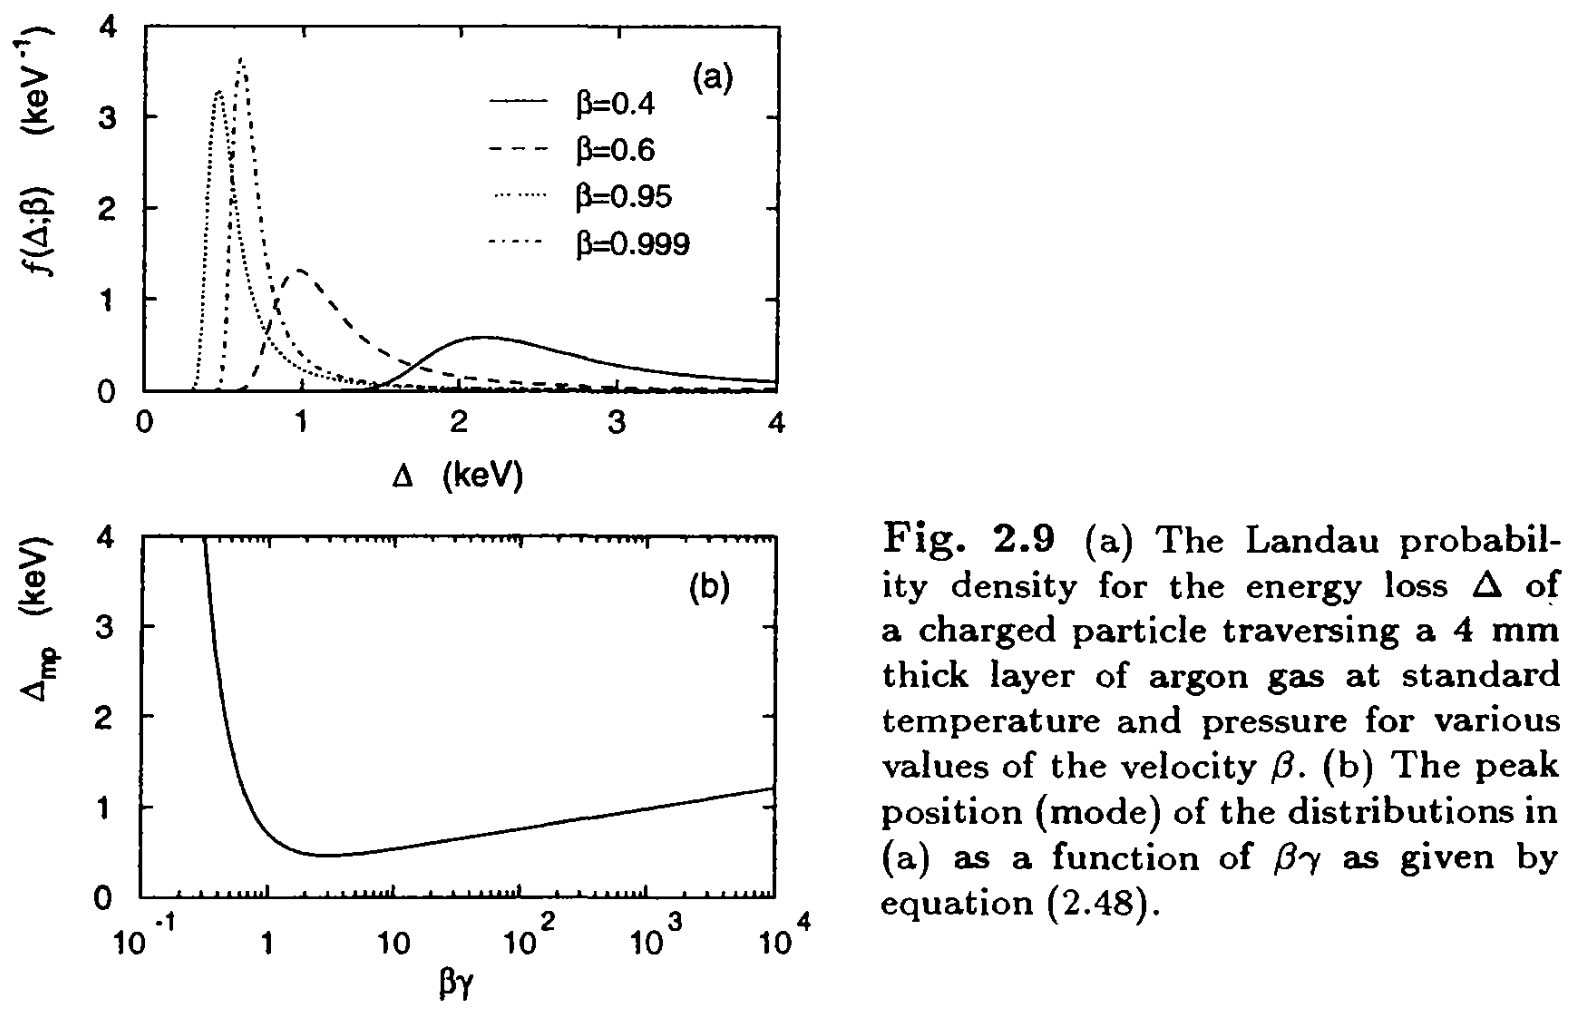
\includegraphics[trim={0cm 0cm 0 0},clip, keepaspectratio,width=0.5\textwidth]{landautails}\label{fig:landautails}\end{figure}
(The model breaks down in the tails of distribution.)
\end{frame}

\begin{frame}{Rayleigh}
\begin{columns}[T]\begin{column}{0.5\textwidth}
x,y RV $N(0,\sigma^2)$
\begin{align*}
&z=\sqrt{x^2+y^2}\\
&f(z)=\frac{z}{\sigma^2}\exp{-\frac{z^2}{2\sigma^2}}\\
&F(z)=1-\exp{-\frac{z^2}{2\sigma^2}}\\
&\mu=\sigma\sqrt{\frac{\pi}{2}},\ \var=(2-\pi/2)\sigma^2
\end{align*}
\end{column}\begin{column}{0.5\textwidth}
\begin{align*}
&f(z)=\int_{x^2+y^2=z^2}\phi(x)\phi(y)\,dx\,dy\\
&=2\pi z\frac{1}{2\pi\sigma^2}\exp{-\frac{z^2}{2\sigma^2}}
\end{align*}
\end{column}\end{columns}
\end{frame}

\begin{frame}{Multivariate gaussian}
\begin{columns}[T]
\begin{column}{0.5\textwidth}
\begin{align*}
&\prob{(\vec{x};\vec{\theta},V)}=\frac{1}{(2\pi)^{N/2}|V|^{1/2}}\exp{-\frac{1}{2}(\vec{x}-\vec{\mu})^TV\expy{-1}(\vec{x}-\vec{\mu})}
\end{align*}
\end{column}
\begin{column}{0.5\textwidth}
Diagonal $\Sigma$ \'e equivalente a n gaussiane. Una gaussiana multivariata si ottiene da n gaussiane $N(0,1)$ tramite trasformazione $X=BZ+\mu$.
\end{column}
\end{columns}
\keyword{Matrice di co-varianza}: $V_{ij}=\E{[(x_i-\mu_i)(x_j-\mu_j)]}$
\end{frame}

\subsection{Chi quadro}\linkdest{chi2}

\begin{frame}{Propriet\'a $\chi^2$}
La distribuzione di chi-squared con $\nu$ gradi di libert\'a $\prob{(\chi_{\nu}^2)}$ \'e la distribuzione di probabilit\'a di $\sum_1^{\nu}x_i^2$ con $x_i\to N(0,1)$ ($\sum_{i=1}^N\frac{(x_i-\mu_i)^2}{\sigma_i^2}$), $\chi^2$ non centrale $x_i\to N(\mu_i,1)$, parametro non centralit\'a $\lambda=\sum\mu_i^2$.
\begin{columns}[T]
	\begin{column}{0.7\textwidth}
Funzione caratteristica: $y=\frac{(x_i-\mu_i)}{\sigma_i}$, $z=y^2$
		\begin{align*}
		&f(z;n=1)=2\phi(y)|\TDy{z}{y}|=\frac{1}{\sqrt{2\pi z}}\exp{-z/2}\\
		&\phi_1(t)=\E_z{(\exp{itz})}=(1-2it)\expy{-1/2}\\
		%&=\intsinf{}\frac{\exp{itx-x^2/2}}{\sqrt{2\pi}}\,dx=\frac{1}{\sqrt{1-2it}},\\
		&\phi_{\chi^2_{\nu}}(t)=(1-2it)\expy{-\frac{\nu}{2}}
		\end{align*}
	\end{column}
	\begin{column}{0.3\textwidth}
		\begin{align*}
		&\E{(\chi^2_{\nu})}=\nu\\
		&\var{[\chi_{\nu}^2]}=2\nu\\
		&\E{(\chi^{2,NC}_{\nu})}=\nu+\lambda
		\end{align*}
	\end{column}
\end{columns}
\begin{align*}
&\prob{(x=\chi^2_{\nu})}=\frac{1}{2\expy{\nu/2}\Gamma(\frac{\nu}{2})}x\expy{\frac{\nu}{2}-1}\exp{-\frac{x^2}{2}}\xrightarrow{\nu\to\infty}N(\nu,2\nu)
\end{align*}
Approssimazione di Fisher: $\prob{(\sqrt{2\chi^2})}\approx N(\sqrt{2\nu-1},1)$
\end{frame}

\section{come lo utilizzo}

\begin{wordonframe}{PDF distanza stelle distribuite uniformemente in x,y,z}
	\begin{block}{Generazione pdf da distribuzione uniforme}
		
	\end{block}
	\begin{columns}
		\begin{column}{0.5\textwidth}
			\begin{block}{Radial Fourier transform}
				\begin{align*}
				&\hat{f}(\vec{k})=\int\exp{-i\scap{k}{x}}f(\vec{x})d^nx\\
				&=s^{\frac{n-2}{2}}\hat{F}_n(s)\\
				&=(2\pi)^{\frac{n}{2}}\int_0^{+\infty}J_{\frac{n-2}{2}}(sr)r^{\frac{n-2}{2}}F(r)r\,dr
				\end{align*}
			\end{block}
		\end{column}
		\begin{column}{0.5\textwidth}
			\begin{block}{MGF of sum of RV is product of their MGF}
				\begin{align*}
				&\MGF{x_i^2}=\E{[\exp{tx_i^2}]}\\
				&=\frac{\sqrt{\pi}[\Erfi{(b\sqrt{t})}-\Erfi{a\sqrt{t}}]}{2(b-a)\sqrt{t}}
				\end{align*}
			\end{block}
		\end{column}
	\end{columns}
	\begin{block}{$(x,y,z)$ distribuite Unif.: $(r,\theta,\phi)$??}
		
	\end{block}
\end{wordonframe}

\end{document}